\documentclass{beamer}
\usepackage[latin1]{inputenc}
\usefonttheme{serif} 
\usefonttheme{structuresmallcapsserif} 

\usetheme{Luebeck}

\usecolortheme[named=magenta]{structure}
\beamertemplatenavigationsymbolsempty
\setbeamertemplate{bibliography item}[text]
\title[Explosions]{Explosions}
\subtitle{Computational Physics Presentation}
\author{Ville, Aapo, Hannu}


\date{April 28, 2015}



\begin{document}

\begin{frame}
\titlepage
\end{frame}

\begin{frame}{Introduction}
\begin{itemize}

\item A nice group project? $\rightarrow$ Do something completely different than during the course
\item Idea: simulate explosions - a non-trivial and fairly interesting subject
\item The actual implementation studies effectively an explosion of gas particles in a vacuum
\item Unrealistic? No - very similar to the intuitive conception of explosions
\item In an explosion the density of the gas that explodes is much higher than that of the surroundings
\item Only when the explosive gas has expanded enough, the surrounding density becomes important - and this regime is not of interest here

\end{itemize}
\end{frame}


\begin{frame}{Physics of an explosion}
\begin{itemize}

\item High density, pressure or temperature with respect to surroundings $\rightarrow$ explosion
\item Start with a high-density gas cloud $\rightarrow$ the physics of the system will take care of the rest
\item Required: fluid dynamics for compressible systems
\item A shock wave should be produced to the progressing explosion front
\item Handling of dynamic length scales: begin with a compressed system and end with an expanded system
\item Only the dynamical properties of the system are studied, so temperature does not require explicit handling

\end{itemize}
\end{frame}

\begin{frame}{Fluid simulation}
\begin{itemize}

\item Simulating the behaviour of a fluid is highly non-trivial
\item Handling a quickly expanding fluid is a non-trivial case within the group of fluid simulations
\item A solution from astrophysics: smoothed particle hydrodynamics
\item Astrophysics is familiar with changing length scales and vacuum boundary conditions - this fits well a simulation of explosions
\item The basic idea is to model the fluid with a group of discrete particles
\item Fluid physics are obtained by applying a smoothing kernel function to the particles

\end{itemize}
\end{frame}

\begin{frame}{SPH basics}
\begin{itemize}

\item Dirac delta function $\delta (\mathbf{x})$ can be approximated using  a kernel function $W(\mathbf{x},h)$ (for instance Gaussian)
\item A function can be represented using delta functions $\rightarrow$
\begin{equation}
 f(\mathbf{x}) = \int_V f(\mathbf{x}') \delta (\mathbf{x}-\mathbf{x}') d\mathbf{x}' \approx \int_V \frac{f(\mathbf{x}')}{\rho(\mathbf{x}')} W(\mathbf{x}-\mathbf{x}',h) \rho(\mathbf{x}') d\mathbf{x}' 
\end{equation}
\item Approximate integral over the density with a sum over point masses:
\begin{equation}
 f(\mathbf{x}) \approx \sum_i m_i \frac{f(\mathbf{x}_i)}{\rho_i} W( \mathbf{x} - \mathbf{x_i}, h )
\end{equation}
\item Now for instance the density can be calculated:
\begin{equation}
\rho(\mathbf{x}) \approx \sum_i m_i W( \mathbf{x} - \mathbf{x_i}, h )
\end{equation}

\end{itemize}
\end{frame}


\begin{frame}{Smoothing kernel functions}
\begin{itemize}

\item Normalized and delta-like, $\int W(\mathbf{r},h) d\mathbf{r} = 1$
\item Gaussian form would be nice, but it goes to zero only at infinite distance
\item We use a commonly utilized cubic spline form that goes to zero at the distance of $2h$
\item Generally, W uses $x = |\mathbf{x} - \mathbf{x}'|/h$ as a parameter and is proportional to $1/h^d$
\item In an explosion the system expands much and it is essential to have adaptive $h$ values
\item At particle locations $\rho h^d = \text{const.}$ is desirable

\end{itemize}
\end{frame}

\begin{frame}{SPH fluid equations}
\begin{itemize}

\item Taking the time derivate of the discrete density turns out to give a discretized version of the
continuity equation
\item Using a hydrodynamical Lagrangian, an equation of motion can be constructed that functions effectively
as the Euler equation
\item Similarly the internal energies could be updated if the temperatures were to be studied
\item An artificial vicous term can be introduced, for instance $\Pi \propto v^2/\rho$ - special form for HE simulations
\item This upgrades the Euler equation to handle better for instance shock fronts (broaden the shock across several h)
\item In a sophisticated implementation also the growth of entropy would be taken into account

\end{itemize}
\end{frame}

\begin{frame}{Recap. of necessary equations}
\begin{itemize}

\item The equation of motion is essential:
\begin{equation}
 \mathbf{a}_i = -\sum_{j \neq i} m_j \left( \frac{P_j}{\rho_j^2} + \frac{P_i}{\rho_i^2} + \Pi_{ij} \right) \nabla_i W_{ij} 
\end{equation}
\item The densities at particle locations are obtained as before:
\begin{equation}
\rho_i = \sum_j m_j W_{ij}
\end{equation}
\item The pressures are obtained from the ideal gas eos.:
\begin{equation}
 P = k \rho^\gamma
\end{equation}
\item Updating $h$ follows from $\rho h^d = \text{const.}$:
\begin{equation}
 \frac{d h_i}{dt} = -\frac{h_i}{\rho d} \sum_{j \neq i} m_j ( \mathbf{v}_i - \mathbf{v}_j ) \cdot \nabla_i W_{ij}
\end{equation}

\end{itemize}
\end{frame}

\begin{frame}{Basic implementation}
\begin{itemize}

\item Begin with a 2D implementation, easy to move to 3D
\item Loop over timesteps and keep updating particle locations, velocities and $h$ values
\item To obtain the changes for $\mathbf{x}$, $\mathbf{v}$ and $h$ densities and pressures need to be calculated
\item An important sub-task is determining the significant neighbors of a particle - these are at most on the distance $2h$
\item A naive implementation goes through all pairs and has $O(N^2)$ complexity, which can be improved
\item EOM. can be handled with the leap-frog algorithm (or e.g. RK)
\item Updates of $h$ can be stabilized with relaxation or with hard reset of the constant value

\end{itemize}
\end{frame}

\begin{frame}{Leap-Frog algorithm}
\begin{itemize}

\item The idea is to stabilize the updating schemes of velocities and locations by updating
velocities and locations that are a half timestep apart
\item This can be expressed so that both the velocities and densities are stored on the same
timestep, but the algorithm still visits half-timestep values:
\begin{eqnarray}
 \mathbf{v}_{i+1/2} = \mathbf{v}_i + \frac{\Delta t}{2} \mathbf{a}_i \\
 \mathbf{r}_{i+1/2} = \mathbf{r}_i + \frac{\Delta t}{2} \mathbf{v}_i
\end{eqnarray}
\item Full steps:
\begin{eqnarray}
\mathbf{v}_{i+1} = \mathbf{v}_i + \Delta t \mathbf{a}_{i+1/2} \\
\mathbf{r}_{i+1} = \mathbf{r}_i + \frac{\Delta t}{2} ( \mathbf{v}_i + \mathbf{v}_{i+1} )
\end{eqnarray}

\end{itemize}
\end{frame}

\begin{frame}{Neighbor list handling}
\begin{itemize}

\item Simple case $O(N^2)$: for each particle loop through particles that are after it in a list -
each pair handled only once
\item Not all particles are used for calculating system properties (e.g. densities) at a certain location
\item When iterating though particles, distances between the current ``center'' and other particles are calculated and too distant particles do not contribute

\end{itemize}
\end{frame}

\begin{frame}{Neighbor list handling}

\begin{figure}[!ht]
\begin{center}
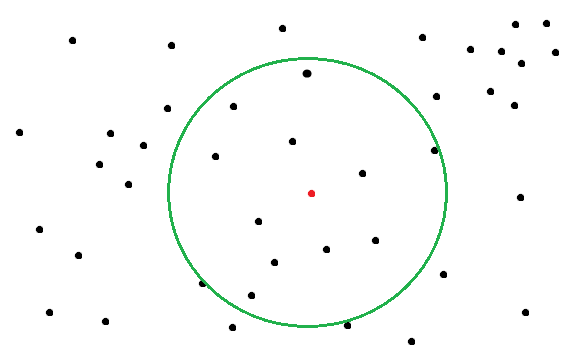
\includegraphics[width=10cm]{N2.png} 

\end{center}
\end{figure}

\end{frame}


\begin{frame}{Neighbor list handling}
\begin{itemize}

\item The distance cutoff for the simple case leads to an intuitive alternative
\item Compartmentalizing  $O(N)$: Form a grid, and create and maintain a list of particles inside each grid box. Then for each particle, find the particle lists of the neighboring grid boxes.
\item Use these lists to solve relevant system properties.
\end{itemize}
\end{frame}

\begin{frame}{Neighbor list handling}

\begin{figure}[!ht]
\begin{center}
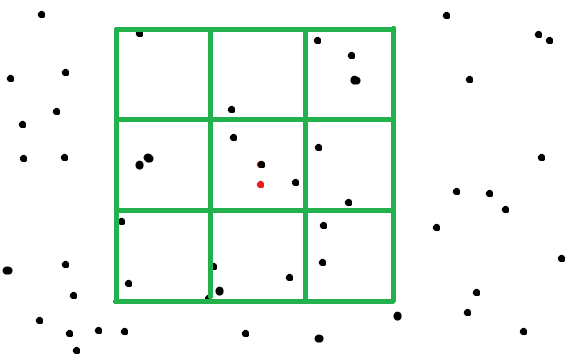
\includegraphics[width=10cm]{N.png} 

\end{center}
\end{figure}

\end{frame}




\begin{frame}{Timestep optimization}
\begin{itemize}

\item Relatively small timesteps are informative, but if the steps are very small the simulation times become lengthy
\item The density and velocities of the particles change during the simulation $\rightarrow$ the optimal timestep?
\item Numerical stability and accuracy vs information lag between the particles $\rightarrow$ global timestep and lockstep evolution (here only CFL and force condition)

\begin{equation}
\delta t_{i} = \min(\delta t_{\rm CFL,i}(h),\delta t_{\rm F,i}(h),\delta t_{\rm RKF,i},\delta t_{\rm 
z,i})
\end{equation}
\begin{equation}
\delta t_{\rm glob} = \min_i{\delta t_i}
\end{equation}

\item Physical meaning: eg. CFL criterion, spatial information transfer speed $<$ local sound speed

\end{itemize}
\end{frame}

\begin{figure}[!ht]
\begin{center}
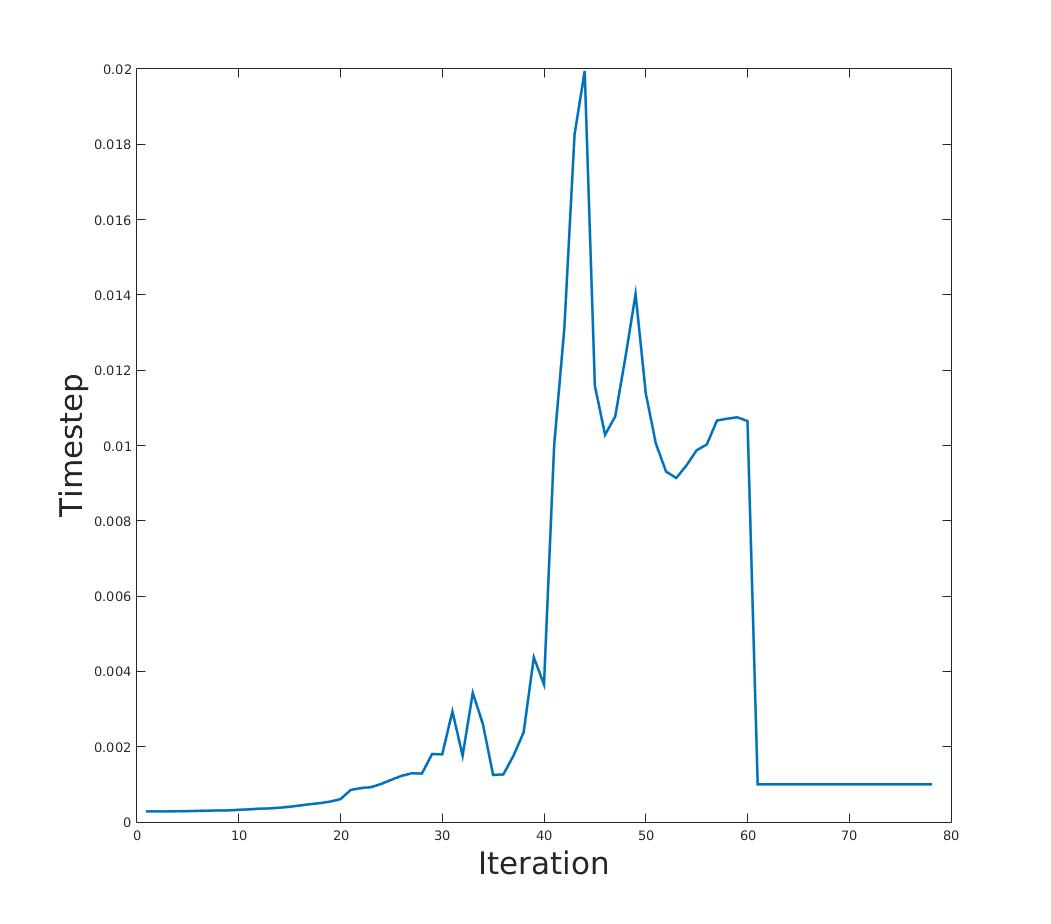
\includegraphics[width=10cm]{tStep_behaviour.jpg} 

\end{center}
\end{figure}


\begin{frame}{First 2D results}
\begin{itemize}

\item Huehuehue

\end{itemize}
\end{frame}

\begin{frame}{References}
\begin{itemize}

\item P. J. Cossins, Smoothed Particle Hydrodynamics, arXiv:1007.1245v2 [astro-ph.IM], 2010 

\item G. R. Liu and M. B. Liu, Smoothed particle hydrodynamics - a meshfree particle method, World Scientific Publishing, Singapore, 2003

\end{itemize}
\end{frame}

\end{document}
